\section{Performance of Annealing-based Quantum Computers}

For the optimization using the Quantum Annealing hardware, the formulated DQM is sent to a hybrid solver at D-Wave.
The hybrid solver does not put the DQM on quantum hardware directly.
It classically searches the solution space.
The hybrid solver speeds up this process by using quantum hardware to determine promising regions to explore next.
\cite{DQMHybrid2020}

The optimization of the DQM using the hybrid solver for small problems seems to have linear time complexity.
Every time $10$ time instances are added to the problem size, the optimization takes about $0.1$ seconds longer.
The results of the optimization and the time needed for the optimization are listed in table \ref{table:validation.annealing.performance}.
The optimization of these problems takes no longer than $5.6$ seconds each.

\todo{redo table. remove 25}

\begin{table}[ht]
  \centering
  \begin{tabular}{| r | r | r |}
  \hline 
  Number of Loads & Objective function & Time (in seconds) \\ 
  \hline \hline 
  10 & 487007.496 & 4.989 \\ \hline 
  20 & 817672.120 & 5.085 \\ \hline 
  25 & 681913.849 & 5.117 \\ \hline 
  30 & 1155685.053 & 5.215 \\ \hline 
  40 & 1554316.529 & 5.362 \\ \hline 
  50 & 1559508.051 & 5.510 \\ \hline 
\end{tabular}

  \caption{Results of annealing optimization with four power plants.}
  \label{table:validation.annealing.performance}
\end{table}

In figure \ref{figure:validation.annealing.performance} the time complexity is displayed clearer.
The time needed for optimizing problems with less than $15$ time instances also seems to be constant.
After that, the linear time complexity is clearly visible.

\begin{figure}[ht]
  \centering
  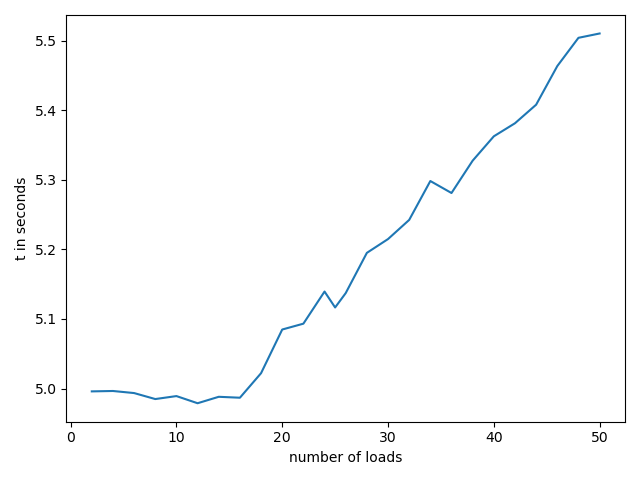
\includegraphics[width=0.75 \textwidth]{04_Validation/performance_annealing_p4.png}
  \caption{Time complexity of annealing optimization with four power plants.}
  \label{figure:validation.annealing.performance}
\end{figure}

This approach does not produce optimal solutions for the UCP.
The summed power output of the single power plants does not meet the power demand because the DQM underestimates the demand part of the UCP.
After retrieving the optimal DQM solution and translating it to a UCP solution, the program adjusts the power outputs of the power plants.
It does so as described in section \ref{approach:annealing.implementation.adjust}.
This leads to a non-optimal solution of the UCP.
